\documentclass[10pt,a4paper]{article}
\usepackage[utf8]{inputenc}
\usepackage{amsmath}
\usepackage{amsfonts}
\usepackage{amssymb}
\usepackage{graphicx}
\usepackage{subfigure}
\usepackage{amsmath}
\usepackage{mathrsfs}
\DeclareRobustCommand{\orderof}{\ensuremath{\mathcal{O}}}
\bibliographystyle{prsty}
\usepackage[top=1in, bottom=1in, left=1in, right=1in]{geometry}

\begin{document}
\section{Introduction}
\textbf{flq\_chn} is a task of extension level. It calculates the Floquet Chern number. To use this task, you must first perform \textbf{flq} first. Most of the keywords are the same with \textbf{chn}, so one should reference \textbf{chn} for details. Also, the attached output data are not complete because they are too large. 

\section{Dictionary}

\subsection{Input}
 The input parameters of \textbf{flq\_chn} share exactly the same keywords as \textbf{chn}. Therefore, one can directly reference the dictionary of \textbf{chn}

\subsection{Output}
\textit{\textbf{flq\_chn.gap\_ind}} This variable gives the location of the band and its band gap. Since Floquet problem has no Fermi level, one can only discuss the Chern number of a particular band gap. This variable gives three column. The first two give the band indies where gap appears and the last one gives its gap energy.\\ \\
The other output data are the same with \textbf{chn}. One should reference \textbf{chn} for details.
 \\ \\
 \\ \\
 \\ \\
 \\ \\
  \\ \\
  \\ \\
 \\ \\
 \\ \\
 \\ \\
 \\ \\
  \\ \\
  \\ \\
  \\ \\
  \\ 
  
  
\begin{figure}[tbp]
\centering
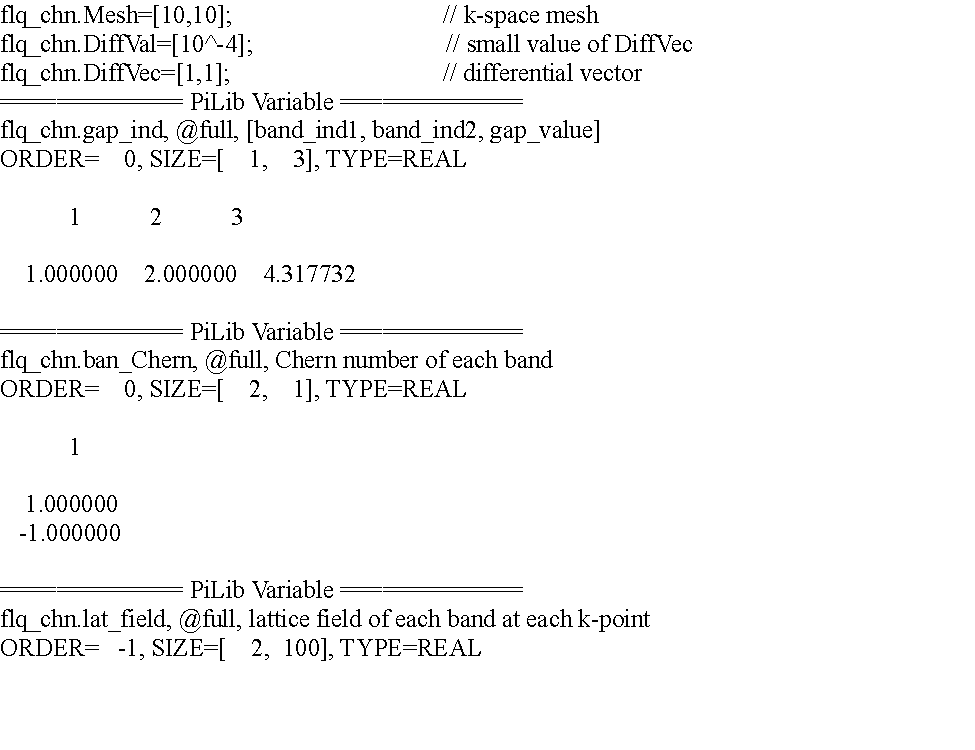
\includegraphics[width=0.9\columnwidth]{Haldane_flq_chn.pdf}
\caption{page 1 of Haldane\_flq\_chn.plb}
\end{figure}

\end{document}